
\begin{frame}[label=hard]{Issue with $c$ unknown}

  \begin{exampleblock}{Summary so far (the \textbf{Easy Case})}
    \begin{itemize}
    \item The \alert{increment} (\alert{c}) is \textbf{known}:
      \begin{itemize}
      \item Remove it, get truncated geometric sequence, CVP.
      \end{itemize}
    \end{itemize}
  \end{exampleblock}
  
  \begin{alertblock}{Now the \textbf{Hard Case}}
    \begin{itemize}
    \item The \alert{increment} (\alert{c}) is \textbf{unknown}:
      \begin{itemize}
      \item How to get truncated geometric sequence?
      \item Use $\Delta S_i = S_{i+1} - S_i \qquad\qquad (\Delta S_{i+1} = a \times \Delta S_i \bmod 2^{128})$.
      \end{itemize}
      \pause
    \item Same attack as before, but...
      \begin{itemize}
    \item Must guess one more rotation.
    \item Must guess least-significant bits of \alert{$c$}.
    \end{itemize}
  \end{itemize}
  \end{alertblock}
\end{frame}

%%%%%%%%%%%%%%%%%%%%%%%%%%%%%%%%%%%%%%%%%%%%%%%%%%%%%%%%%%%%%


\begin{frame}[label=hard_dtl]{Attack Details}

\begin{figure}
\begin{center}
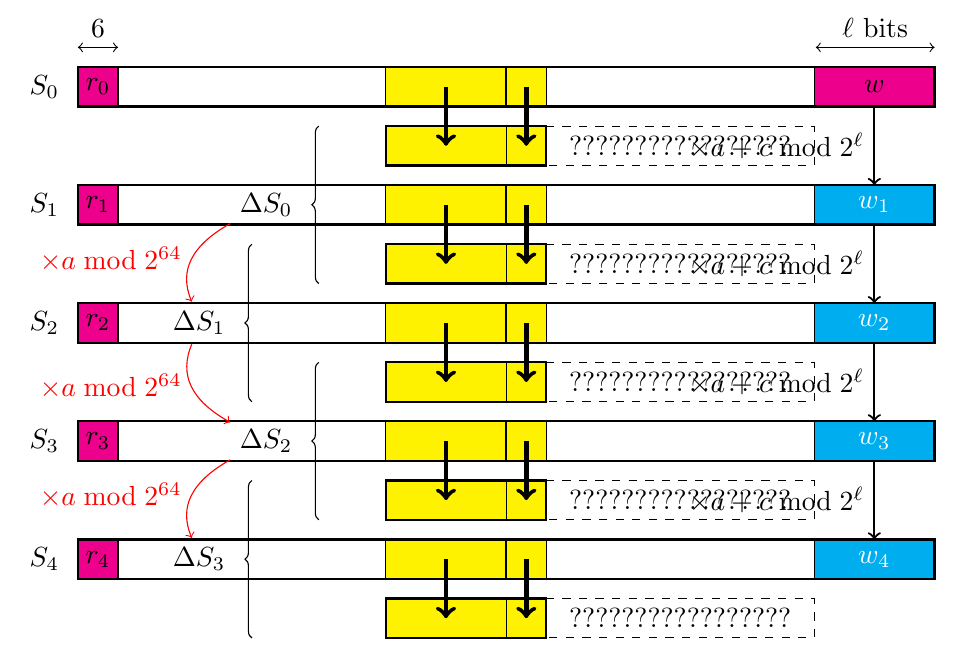
\begin{tikzpicture}[xscale=0.85, yscale=0.5]
  \path[red, use as bounding box] (-0.75, -13.5) rectangle (12.8, 2);
  
  % S_0
  \begin{scope}
    % remplissage
    \fill<4-5>[fill=yellow] (4.6, 0) rectangle +(2.4, 1);
    \fill<2-5>[fill=magenta] (0, 0) rectangle node {$r_0$} +(0.6, 1);
    \fill<2-5>[fill=magenta] (11, 0) rectangle node {$w$} +(1.8, 1);
    
    % bordures
    \draw<1-5>[thick]  (0, 0) rectangle (12.8, 1);
    \draw<2-5>  (0.6, 0) rectangle +(0, 1);
    \draw<1-5>[thick]  (6.4, 0) rectangle +(0, 1);
    \draw<4-5>  (7.0, 0) rectangle +(0, 1);
    \draw<4-5> (4.6, 0) rectangle +(0, 1);
    \draw<2-5>  (11, 0) rectangle +(0, 1);
    
    % déco autour
    \node<1-5> at (-0.5, 0.5) {$S_0$};
    \draw<2-5>[<->] (12.8, 1.5) -- node[above] {$\ell$ bits} +(-1.775, 0);
    \draw<2-5>[<->] (0, 1.5) -- node[above] {6} +(0.6, 0);
  \end{scope}

  % T_0
  \begin{scope}[xshift=4.6cm, yshift=-1.5cm]    
    \draw<5->[dashed]  (0, 0) rectangle +(6.4, 1);
    \draw<5->[thick,fill=yellow]   (0, 0) rectangle +(2.4, 1);
    \draw<5>[]   (1.8, 0) rectangle +(0, 1);
    \path<5->  (2.4, 0) rectangle node {$?????????????????$} (6.4, 1);
  \end{scope}

  % flèches S_i --> T_i
  \draw<5> [ultra thick,->] (5.5, 0.5) -- +(0, -1.5);
  \draw<5> [ultra thick,->] (6.7, 0.5) -- +(0, -1.5);

  
  %%%%%%%%%

  
  % S_1
  \begin{scope}[yshift=-3cm]
    % remplissage
    \fill<4-5>[fill=yellow] (4.6, 0) rectangle +(2.4, 1);
    \fill<2-5>[fill=magenta] (0, 0) rectangle node {$r_1$} +(0.6, 1);
    \fill<3-5>[fill=cyan] (11, 0) rectangle node[text=white] {$w_1$} +(1.8, 1);
    
    % bordures
    \draw<1-5>[thick]  (0, 0) rectangle (12.8, 1);
    \draw<2-5>  (0.6, 0) rectangle +(0, 1);
    \draw<1-5>[thick]  (6.4, 0) rectangle +(0, 1);
    \draw<4-5>  (7.0, 0) rectangle +(0, 1);
    \draw<4-5>  (4.6, 0) rectangle +(0, 1);
    \draw<3-5>  (11, 0) rectangle +(0, 1);
    
    % déco autour
    \node<1-5> at (-0.5, 0.5) {$S_1$};
  \end{scope}
  
  % T_1
  \begin{scope}[xshift=4.6cm, yshift=-4.5cm]    
    \draw<5->[dashed]  (0, 0) rectangle +(6.4, 1);
    \draw<5->[thick,fill=yellow]  (0, 0) rectangle +(2.4, 1);
    \draw<5>[]  (1.8, 0) rectangle +(0, 1);
    \path<5-> (2.4, 0) rectangle node {$?????????????????$} (6.4, 1);
  \end{scope}

  \begin{scope}[yshift=-3cm]
    % flèches S_i --> T_i
    \draw<5>[ultra thick,->] (5.5, 0.5) -- +(0, -1.5);
    \draw<5>[ultra thick,->] (6.7, 0.5) -- +(0, -1.5);
  \end{scope}

  
  %%%%%%%%%%%%%

  
  % S_2
  \begin{scope}[yshift=-6cm]
    % remplissage
    \fill<4-5>[fill=yellow] (4.6, 0) rectangle +(2.4, 1);
    \fill<2-5>[fill=magenta] (0, 0) rectangle node {$r_2$} +(0.6, 1);
    \fill<3-5>[fill=cyan] (11, 0) rectangle node[text=white] {$w_2$} +(1.8, 1);
    
    % bordures
    \draw<1-5>[thick]  (0, 0) rectangle (12.8, 1);
    \draw<2-5>  (0.6, 0) rectangle +(0, 1);
    \draw<1-5>[thick]  (6.4, 0) rectangle +(0, 1);
    \draw<4-5>  (7.0, 0) rectangle +(0, 1);
    \draw<4-5>  (4.6, 0) rectangle +(0, 1);
    \draw<3-5>  (11, 0) rectangle +(0, 1);
    
    % déco autour
    \node<1-5> at (-0.5, 0.5) {$S_2$};
  \end{scope}    
  
  % T_2
  \begin{scope}[xshift=4.6cm, yshift=-7.5cm]    
    \draw<5->[dashed]  (0, 0) rectangle +(6.4, 1);
    \draw<5->[thick,fill=yellow]  (0, 0) rectangle +(2.4, 1);
    \draw<5>[]  (1.8, 0) rectangle +(0, 1);
    \path<5-> (2.4, 0) rectangle node {$?????????????????$} (6.4, 1);
  \end{scope}

  \begin{scope}[yshift=-6cm]
    % flèches S_i --> T_i
    \draw<5>[ultra thick,->] (5.5, 0.5) -- +(0, -1.5);
    \draw<5>[ultra thick,->] (6.7, 0.5) -- +(0, -1.5);
  \end{scope}

  
  %%%%%%%%%%%%%

  
  % S_3
  \begin{scope}[yshift=-9cm]
    % remplissage
    \fill<4-5>[fill=yellow] (4.6, 0) rectangle +(2.4, 1);
    \fill<2-5>[fill=magenta] (0, 0) rectangle node {$r_3$} +(0.6, 1);
    \fill<3-5>[fill=cyan] (11, 0) rectangle node[text=white] {$w_3$} +(1.8, 1);
    
    % bordures
    \draw<1-5>[thick]  (0, 0) rectangle (12.8, 1);
    \draw<2-5>  (0.6, 0) rectangle +(0, 1);
    \draw<1-5>[thick]  (6.4, 0) rectangle +(0, 1);
    \draw<4-5>  (7.0, 0) rectangle +(0, 1);
    \draw<4-5>  (4.6, 0) rectangle +(0, 1);
    \draw<3-5>  (11, 0) rectangle +(0, 1);
    
    % déco autour
    \node<1-5> at (-0.5, 0.5) {$S_3$};
   \end{scope}

  % T_3
  \begin{scope}[xshift=4.6cm, yshift=-10.5cm]    
    \draw<5->[dashed]  (0, 0) rectangle +(6.4, 1);
    \draw<5->[thick,fill=yellow]  (0, 0) rectangle +(2.4, 1);
    \draw<5>[]  (1.8, 0) rectangle +(0, 1);
    \path<5-> (2.4, 0) rectangle node {$?????????????????$} (6.4, 1);
  \end{scope}

  \begin{scope}[yshift=-9cm]
  % flèches S_i --> T_i
    \draw<5>[ultra thick,->] (5.5, 0.5) -- +(0, -1.5);
    \draw<5>[ultra thick,->] (6.7, 0.5) -- +(0, -1.5);
  \end{scope}
  
    %%%%%%%%%%%%%

  
  % S_4
  \begin{scope}[yshift=-12cm]
    % remplissage
    \fill<4-5>[fill=yellow] (4.6, 0) rectangle +(2.4, 1);
    \fill<2-5>[fill=magenta] (0, 0) rectangle node {$r_4$} +(0.6, 1);
    \fill<3-5>[fill=cyan] (11, 0) rectangle node[text=white] {$w_4$} +(1.8, 1);
    
    % bordures
    \draw<1-5>[thick]  (0, 0) rectangle (12.8, 1);
    \draw<2-5>  (0.6, 0) rectangle +(0, 1);
    \draw<1-5>[thick]  (6.4, 0) rectangle +(0, 1);
    \draw<4-5>  (7.0, 0) rectangle +(0, 1);
    \draw<4-5>  (4.6, 0) rectangle +(0, 1);
    \draw<3-5>  (11, 0) rectangle +(0, 1);
    
    % déco autour
    \node<1-5> at (-0.5, 0.5) {$S_4$};
  \end{scope}    

  % T_4
  \begin{scope}[xshift=4.6cm, yshift=-13.5cm]    
    \draw<5->[dashed]  (0, 0) rectangle +(6.4, 1);
    \draw<5->[thick,fill=yellow]  (0, 0) rectangle +(2.4, 1);
    \draw<5>[]  (1.8, 0) rectangle +(0, 1);
    \path<5-> (2.4, 0) rectangle node {$?????????????????$} (6.4, 1);
  \end{scope}
  \begin{scope}[yshift=-12cm]
  % flèches S_i --> T_i
    \draw<5>[ultra thick,->] (5.5, 0.5) -- +(0, -1.5);
    \draw<5>[ultra thick,->] (6.7, 0.5) -- +(0, -1.5);
  \end{scope}

  
  % Differences
  \begin{scope}[xshift=4.6cm, decoration={brace,mirror},>=stealth]  
    \draw<6>[decorate]  (-1, -0.5) -- +(0, -4);
    \node<6>[anchor=east] at (-1.25, -2.5)  (T0) {$\Delta S_0$};
  \end{scope}

  % Differences
  \begin{scope}[xshift=3.6cm, yshift=-3cm, decoration={brace,mirror},>=stealth]  
    \draw<6>[decorate]  (-1, -0.5) -- +(0, -4);
    \node<6>[anchor=east] at (-1.25, -2.5)  (T1) {$\Delta S_1$};
  \end{scope}

  % Differences
  \begin{scope}[xshift=4.6cm, yshift=-6cm, decoration={brace,mirror},>=stealth]  
    \draw<6>[decorate]  (-1, -0.5) -- +(0, -4);
    \node<6>[anchor=east] at (-1.25, -2.5)  (T2) {$\Delta S_2$};
  \end{scope}

  % Differences
  \begin{scope}[xshift=3.6cm, yshift=-9cm, decoration={brace,mirror},>=stealth]  
    \draw<6>[decorate]  (-1, -0.5) -- +(0, -4);
    \node<6>[anchor=east] at (-1.25, -2.5)  (T3) {$\Delta S_3$};
  \end{scope}

  % arrows
  \draw<6>[red,->] (T0) edge[bend right] node[left] {$\times a \bmod 2^{64}$} (T1);
  \draw<6>[red,->] (T1) edge[bend right] node[left] {$\times a \bmod 2^{64}$} (T2);
  \draw<6>[red,->] (T2) edge[bend right] node[left] {$\times a \bmod 2^{64}$} (T3);

  % flèches w
  \draw<3>[thick,->] (11.9, 0) -- node[left] {$\times a + c \bmod \alert{2^\ell}$} +(0, -2);
  \draw<3>[thick,->] (11.9, -3) -- node[left] {$\times a + c \bmod \alert{2^\ell}$} +(0, -2);
  \draw<3>[thick,->] (11.9, -6) -- node[left] {$\times a + c \bmod \alert{2^\ell}$} +(0, -2);
  \draw<3>[thick,->] (11.9, -9) -- node[left] {$\times a + c \bmod \alert{2^\ell}$} +(0, -2);
  
\end{tikzpicture}
\end{center}
\end{figure}
\end{frame}

%%%%%%%%%%%%%%%%%%%%%%%%%%%%%%%%%%%%%%%%%%%%%%%%%%%%%%%%%%%%

\begin{frame}<1>[label=hard_test]{Attack Details (cont'd)}

  \begin{block}{Summary so far}
    \begin{itemize}
    \item \textbf{Guess} parts of the states ($S_i$).
    \item Attack state \textbf{differences} ($\Delta S_i$).
    \item CVP in dim. 4 $\leadsto$ reconstruct partial $\Delta S_i \qquad$ (for all $i$).
    \end{itemize}
  \end{block}

  \bigskip

  \begin{alertblock}{Problem}
    How to check if guesses are valid?
  \end{alertblock}

  \bigskip
  \pause

  \begin{exampleblock}{Solution}
    \begin{itemize}
    \item $\color{cyan} S_i[64:64+\ell]$ from guesses + $X_i$ (output) + $r_i$ (rotation).
    \item $\color{orange} S_i[64:64+\ell]$ from guesses + partial $\Delta S_i$.
    \item[$\Rightarrow$] Try all possible $r_i$'s. No match $\leadsto$ bad guess.
    \end{itemize}
  \end{exampleblock}
\end{frame}


%%%%%%%%%%%%%%%%%%%%%%%%%%%%%%%%%%%%%%%%%%%%%%%%%%%%%%%%%%%%

\begin{frame}[label=hard_test_dtl]{Consistency Check}

%  For any future state $S_i$:
  
  %for $0 \leq r \leq 63$
    \begin{center}
    \begin{tikzpicture}[scale=0.5,>=stealth]
      \path[red, use as bounding box] (-8, -6.5) rectangle (12.8, 7);

      % S_0
      \node<2-> at (-6.3, 5.5) {$S_0$};
      \draw<2->[very thick]  (-5.8, 5) rectangle +(18.6, 1);
      \draw<2->[very thick,fill=orange] (0, 5) rectangle +(3.5, 1);

      % Delta S_i
      \node<2-> at (-6.6, 4) {$\Delta S_i$};
      \draw<2->[very thick]  (-5.8, 3.5) rectangle +(18.6, 1);
      \draw<2->[very thick,fill=orange] (0, 3.5) rectangle +(3.5, 1);


      \node<3-> at (-8, 2.5) (add) {\scalebox{1.5}{$\boxplus$}};
      \draw<3->[->] (1.75, 6) -- (1.75, 7) -- (-8, 7) -- (add);
      \draw<3->[->] (1.75, 3.5) -- (1.75, 2.5) -- (add);
      \draw<3->[->] (add) -- (-8, 1) -- (1.75, 1) -- (1.75, 0.1);

      \begin{scope}[yshift=-1cm]
      
        % S_i
        \node at (-6.3, 0.5) {$S_i$};
        \draw[very thick]  (-5.8, 0) rectangle +(18.6, 1);
        \fill<3->[pattern=north east lines, pattern color=orange] (0, 0) rectangle +(3.5, 1);
        \fill<5->[pattern=north west lines, pattern color=cyan]   (0, 0) rectangle +(3.5, 1);
        \draw[very thick] (0, 0) rectangle +(3.5, 1);
        \draw<4->[very thick,fill=cyan] (9.3, 0) rectangle (12.8, 1);
        
        \node[font=\footnotesize] at (12.8, -0.33) {$0$};
        \node[font=\footnotesize] at (3.5, -0.33) {$64$};
        
        \node[font=\footnotesize] at (-0.25, -0.33) {$64 +\ell$ };
%        \node[font=\footnotesize] at (-6, -0.33) {$128$};
        
        \draw<5-> (6.4, -2) node (x) {$\bigoplus$};
        
        \draw<5->[<-] (1.75, -0.1) |- (x);
        \draw<5->[->] (11.2, -0.0) |- (x);
        \draw<5->[<-] (x) --  (6.4, -4.3);
        
        % X_i
        \begin{scope}[xshift=-1.15cm]
        \node<4->[anchor=east] at (0, -4.8) {$X_i \lll r_i$};
        \draw<4->[very thick]  (0, -4.3) rectangle +(9.3, -1);
        \draw<4->[very thick,fill=cyan]  (9.3, -4.3) rectangle +(-3.5, -1);
      \end{scope}
    \end{scope}
  \end{tikzpicture}
    \end{center}
\end{frame}

\againframe<2>{hard_test}

% \begin{frame}{Complete State Reconstruction}
% \begin{itemize}
%     \item We get the Full Difference:
%     \begin{itemize}
%         \item We recover the 63 first rotations
%         \item $\Delta S_i[122:128] = r_{i+1} - r_{i}$
%         \item $\Delta S = CVP(2^{122} \Delta S[122:128],\mathcal{L})$
%     \end{itemize}
%     \item  We deduce the entire $S_0$
%     \begin{itemize}
%         \item probably could have used a SAT-solver
%         \item we recover $S_0$ from right to left by computing the carries
%     \end{itemize}
% \end{itemize}
% \end{frame}


%%%%%%%%%%%%%%%%%%%%%%%%%%%%%%%%%%%%%%%%%%%%%%%%%%%%%%%%%%%%

\begin{frame}<1>[label=hard_finish]{Finishing it Off}

  \begin{block}{Summary so far}
    \begin{itemize}
    \item \textbf{Guessed} parts of the states ($S_i$).
    \item Isolated \textbf{correct} guess $\leadsto$ correct partial differences $\Delta S_i$.
    \end{itemize}
  \end{block}

  \bigskip

  \begin{alertblock}{Problem}
    How to get full initial state $S_0$?
  \end{alertblock}

  \bigskip
  \pause

  \begin{exampleblock}{Solution}
    \begin{itemize}
    \item Correct partial $\Delta S_i$ + consistency check $\leadsto$ \textbf{all} rotations $r_i$.
    \item[$\Rightarrow$] MSB of all $S_i$ $\leadsto$ MSB of all $\Delta S_i$.
    \item[$\Rightarrow$] CVP in dim. 64 $\leadsto$ full $\Delta S_0$.
      \pause
    \item The rest is easy.
    \end{itemize}
  \end{exampleblock}
\end{frame}


\againframe<5>{hard_test_dtl}
\againframe<2>{hard_finish}


\begin{frame}[label=hard_big_cvp]{Reconstructing the Full Differences (CVP in dim. 64)}
  \begin{center}
    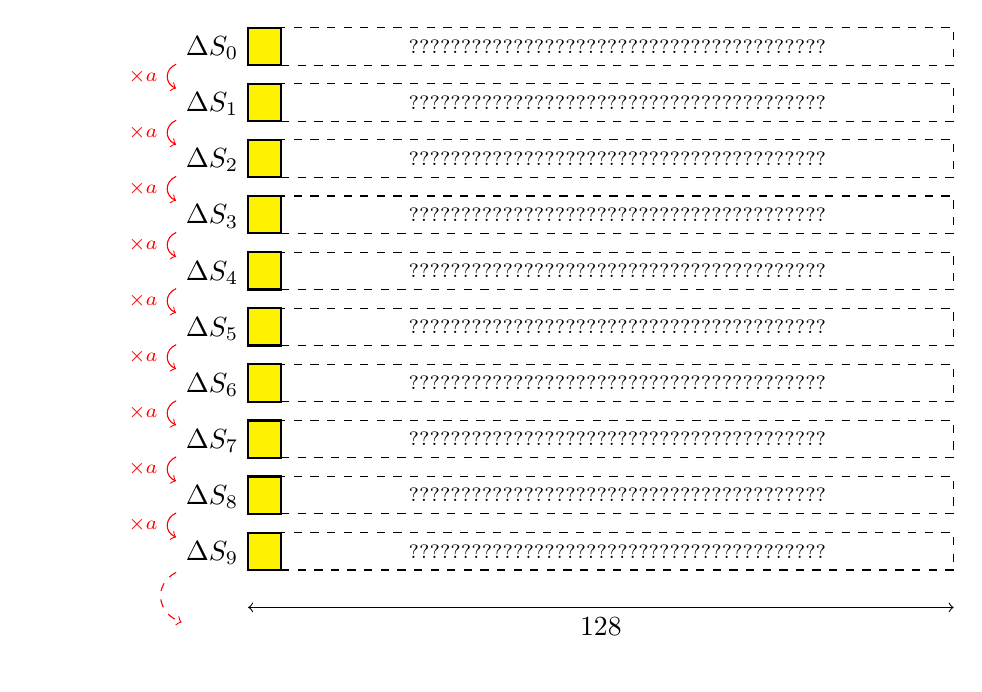
\begin{tikzpicture}[xscale=0.7, yscale=0.475]
      \path[red, use as bounding box] (-4, -16) rectangle (12.8, 1);
      
      
      % T_0
      \foreach \i in {0, 1, ..., 9} {
        \begin{scope}[yshift=-\i*1.5cm]    
          \draw[dashed]  (0, 0) rectangle +(12.8, 1);
          \draw[thick,fill=yellow]  (0, 0) rectangle +(0.6, 1);
          \path (0.6, 0) rectangle node[font=\scriptsize] {$????????????????????????????????????????$} (12.8, 1);
          \node [anchor=east] at (0, 0.45) (DS_\i) {$\Delta S_{\i}$};
        \end{scope}
      }
      
        \begin{scope}[yshift=-10.5*1.5cm]    
          \node [anchor=east] at (0.3, 0.45) (DS_10) {\phantom{$\Delta S_{11}$}};
        \end{scope}

      
      % arrows
      \draw[red,->] (DS_0) edge[bend right=2cm] node[left,font=\scriptsize] {$\times a$} (DS_1);
      \draw[red,->] (DS_1) edge[bend right=2cm] node[left,font=\scriptsize] {$\times a$} (DS_2);
      \draw[red,->] (DS_2) edge[bend right=2cm] node[left,font=\scriptsize] {$\times a$} (DS_3);
      \draw[red,->] (DS_3) edge[bend right=2cm] node[left,font=\scriptsize] {$\times a$} (DS_4);
      \draw[red,->] (DS_4) edge[bend right=2cm] node[left,font=\scriptsize] {$\times a$} (DS_5);
      \draw[red,->] (DS_5) edge[bend right=2cm] node[left,font=\scriptsize] {$\times a$} (DS_6);
      \draw[red,->] (DS_6) edge[bend right=2cm] node[left,font=\scriptsize] {$\times a$} (DS_7);
      \draw[red,->] (DS_7) edge[bend right=2cm] node[left,font=\scriptsize] {$\times a$} (DS_8);
      \draw[red,->] (DS_8) edge[bend right=2cm] node[left,font=\scriptsize] {$\times a$} (DS_9);
      \draw[red,->,dashed] (DS_9) edge[bend right=2cm] (DS_10);

      % size
      \draw[<->] (0, -14.5) -- node[below] {128} +(12.8, 0);
    \end{tikzpicture}
  \end{center}
\end{frame}

\againframe<3>{hard_finish}

%%% Local Variables:
%%% mode: latex
%%% TeX-master: "../main"
%%% End:
